\documentclass[11pt]{article}

\usepackage[letterpaper,margin=0.72in,headheight=15pt]{geometry}
\usepackage{amssymb}
\usepackage{array}
\usepackage{booktabs}
\usepackage{fancyhdr}
\usepackage{graphicx}
\usepackage{listings}
\usepackage{microtype}
\usepackage{tabularx}
\usepackage{tikz}
\usepackage{xcolor}
\usepackage[hidelinks]{hyperref}

\usetikzlibrary{arrows.meta,positioning,shapes.geometric}
\graphicspath{{docs/lessons/assets/}{../assets/}}

\definecolor{ink}{HTML}{20252A}
\definecolor{soft}{HTML}{F1F1EE}
\definecolor{mid}{HTML}{747B80}
\definecolor{accent}{HTML}{405B67}
\definecolor{codebg}{HTML}{F5F5F2}

\pagestyle{fancy}
\fancyhf{}
\lhead{\textsc{ADK field lesson 001}}
\rhead{Mega 2560 built-in LED}
\cfoot{\thepage}
\setlength{\parindent}{0pt}
\setlength{\parskip}{5pt}
\renewcommand{\arraystretch}{1.22}

\lstdefinestyle{adkcpp}
{
    language=C++,
    basicstyle=\ttfamily\small,
    backgroundcolor=\color{codebg},
    frame=single,
    rulecolor=\color{mid},
    columns=fullflexible,
    keepspaces=true,
    showstringspaces=false,
    keywordstyle=\bfseries\color{accent},
    commentstyle=\itshape\color{mid},
    breaklines=true,
    tabsize=4
}

\newcommand{\blankline}{\rule{0.96\linewidth}{0.35pt}}
\newcommand{\checkbox}{\(\square\)}
\newcommand{\statebox}[3]{%
    \begin{tikzpicture}[baseline=(current bounding box.center)]
        \node[draw,rounded corners=2pt,minimum width=1.8cm,minimum height=0.62cm,
              fill=#2,align=center] (#1) {\textbf{#3}};
    \end{tikzpicture}}

\newenvironment{checkpoint}[1]
{\begin{center}\begin{minipage}{0.94\linewidth}\color{ink}\textbf{Check --- #1}\par}
{\end{minipage}\end{center}}

\begin{document}

\begin{center}
    {\Huge\bfseries Make one light become evidence}\\[3pt]
    {\Large Lesson 001: the Mega 2560 built-in LED}\\[8pt]
    \textit{Predict $\rightarrow$ command $\rightarrow$ observe $\rightarrow$ explain}
\end{center}

\begin{center}
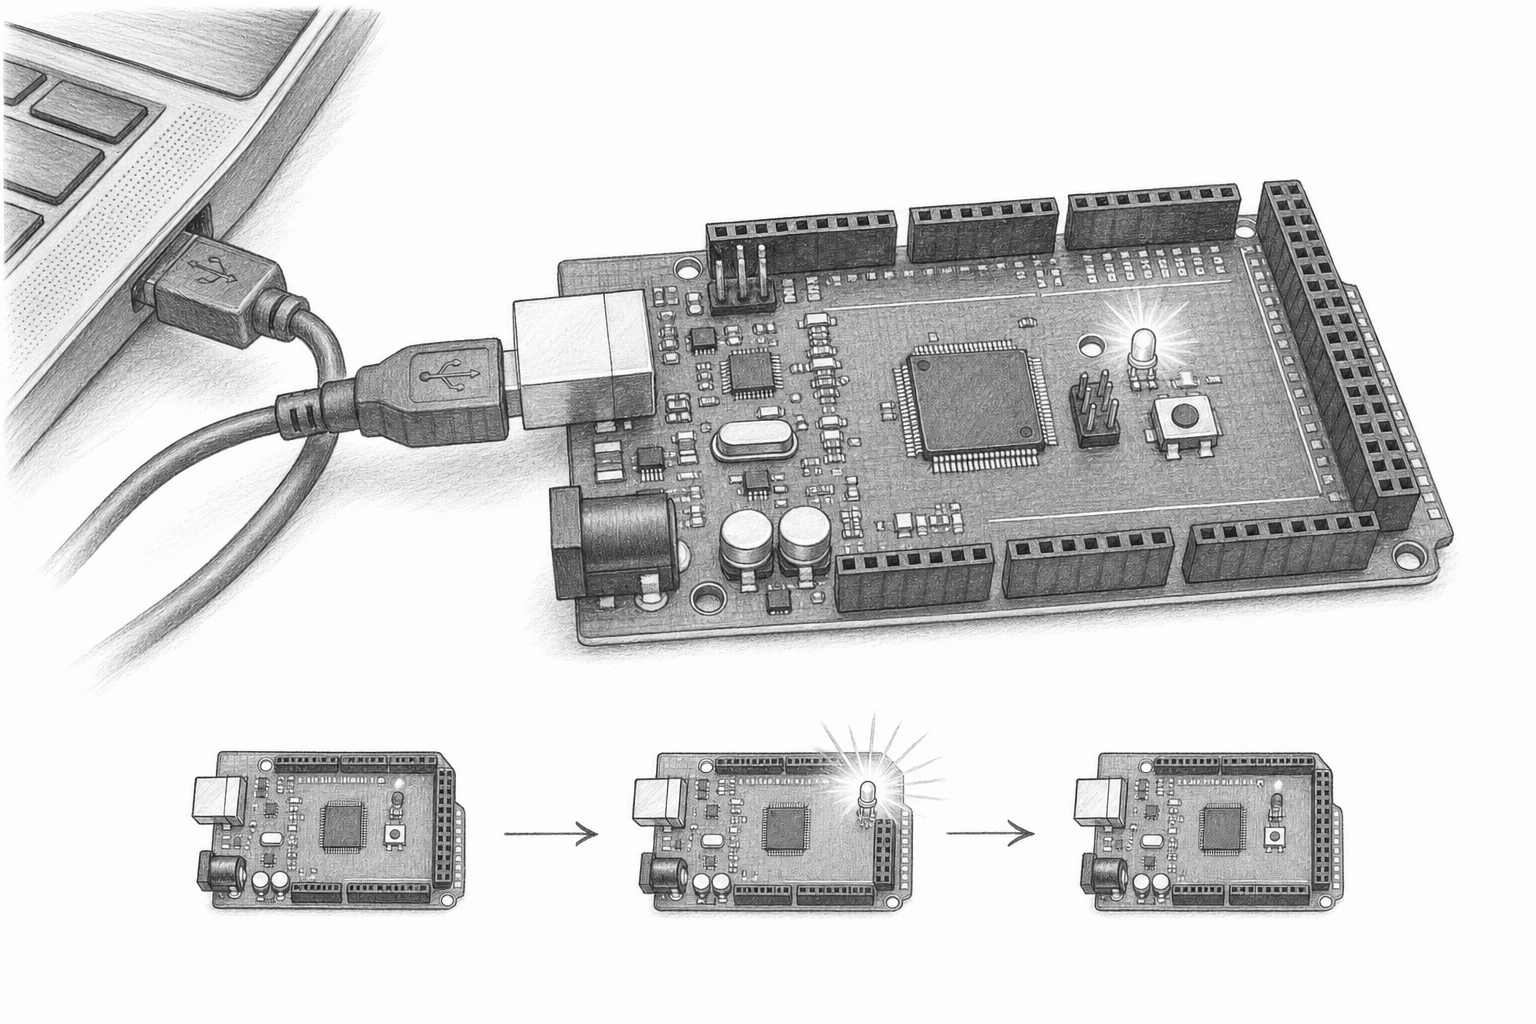
\includegraphics[width=\linewidth,height=0.35\textheight,keepaspectratio]
    {001-built-in-led-pencil.png}
\end{center}

\textbf{Teaching job of the plate.}
Use this graphite view only to orient the board, USB cable, and changing light.
It is an observational illustration, not a pin map or circuit measurement.
Its prominent lamp is symbolic: the Mega 2560 does not require the learner to
find, touch, or wire a literal through-hole LED shown in this plate.
The exact logic used in this lesson appears in the vector diagrams below.
The Mega's built-in indicator is conventionally addressed by
\texttt{LED\_BUILTIN}; do not infer a pin from the drawing.

\begin{tabularx}{\linewidth}{@{}>{\bfseries}lX@{}}
Question & Can a C++ object make the board's own LED produce a repeatable,
testable timing pattern?\\
Time & 35--50 minutes, plus one controlled extension\\
You need & Arduino Mega 2560, known-good USB data cable, Arch Linux computer,
\texttt{arduino-cli}, this ADK checkout\\
You do not need & Breadboard, jumper wires, resistor, external LED, battery,
or RF equipment\\
Proof of success & At least three complete cycles observed, a timing record,
and a claim supported by evidence and reasoning\\
\end{tabularx}

\section*{Safety boundary and stop conditions}

This lesson uses only the board's factory-installed LED and USB power.
Work on a dry, nonconductive surface. Remove jewelry that could bridge
conductors. Keep loose metal away from headers. Never connect USB and an
unknown external power source at the same time.

\textbf{All-power-off setup check:} disconnect USB, barrel-jack power, anything
on \texttt{VIN}, batteries, shields, and every external lead before inspection.
Do not assume removing USB de-energizes a previously assembled board. Confirm
that no power source remains, then inspect the bare board and cable. Proceed
only if the board is dry and has no scorched area, loose metal, bent pins
touching one another, or damaged USB connector.

\textbf{Stop immediately} if a component becomes hot, smoke or odor appears,
the power LED flickers unexpectedly, the USB connector is loose, or the host
reports repeated over-current disconnects. Remove power at its upstream
source---USB at the computer end and any other source, if one is unexpectedly
present and can be disconnected safely. Do not touch a hot or damaged board
and do not ``try once more.'' Mark it \textsc{do not use} and escalate to a
qualified maintainer.

\begin{checkpoint}{record the all-power-off inspection before applying power}
Board ID or label: \rule{4.0cm}{0.35pt}\qquad
Date/time: \rule{3.2cm}{0.35pt}

\checkbox\ every power source removed \quad \checkbox\ bare board dry \quad
\checkbox\ no visible damage \quad \checkbox\ headers clear \quad
\checkbox\ cable sound
\end{checkpoint}

\section*{1. Predict before running}

The supplied program commands the LED on for 100 ms and off for 100 ms.
Complete the prediction without uploading.

\begin{center}
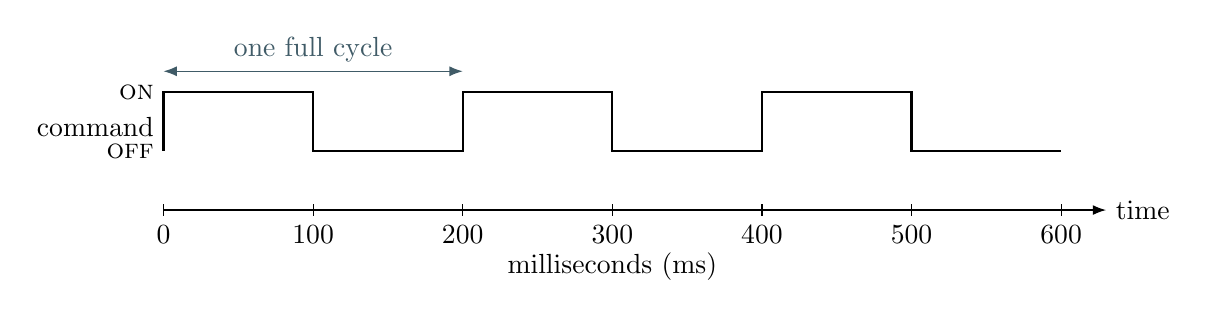
\begin{tikzpicture}[x=0.95cm,y=0.75cm,>=Latex]
    \draw[->] (0,0) -- (12.6,0) node[right]{time};
    \foreach \x/\lab in {0/0,2/100,4/200,6/300,8/400,10/500,12/600}
    {
        \draw (\x,0.10) -- (\x,-0.10) node[below]{\lab};
    }
    \node[left] at (0,1.4) {command};
    \draw[thick] (0,1) -- (0,2) -- (2,2) -- (2,1) -- (4,1)
                 -- (4,2) -- (6,2) -- (6,1) -- (8,1)
                 -- (8,2) -- (10,2) -- (10,1) -- (12,1);
    \node[left] at (0,2) {\textsc{on}};
    \node[left] at (0,1) {\textsc{off}};
    \node[below] at (6,-0.55) {milliseconds (ms)};
    \draw[<->,accent] (0,2.35) -- node[above]{one full cycle} (4,2.35);
\end{tikzpicture}
\end{center}

\textbf{Prediction A.} One full cycle lasts
\rule{1.4cm}{0.35pt} ms. In seconds this is
\rule{1.4cm}{0.35pt} s.

\textbf{Prediction B.} Expected cycles per second:
\[
f=\frac{1}{T}=\frac{1}{\rule{2.2cm}{0.35pt}\ {\rm s}}
=\rule{2.2cm}{0.35pt}\ {\rm cycles/s}.
\]

\textbf{Prediction C.} During a 10 s observation, I expect approximately
\rule{2cm}{0.35pt} complete cycles. I expect the LED to appear
\(\square\) clearly blinking \quad \(\square\) steadily lit \quad
\(\square\) steadily dark.

\textit{Commit before revealing the worked example:}
Why might your eyes give weaker timing evidence than the program text?
\par\noindent\blankline

\subsection*{Worked example, with units}

The two delays make
\[
T=100\ {\rm ms}+100\ {\rm ms}=200\ {\rm ms}
  \left(\frac{1\ {\rm s}}{1000\ {\rm ms}}\right)=0.200\ {\rm s}.
\]
Therefore
\[
f=\frac{1}{0.200\ {\rm s}}=5.00\ {\rm s}^{-1}=5.00\ {\rm Hz}.
\]
Ten seconds should contain about \(10\ {\rm s}\times5.00\ {\rm s}^{-1}=50\)
cycles. That is the \emph{commanded} pattern. The time spent executing calls
and loop instructions, the board clock's tolerance, and human reaction time
make a hand-timed observation less exact.

\section*{2. Three representations of the same experiment}

\begin{center}
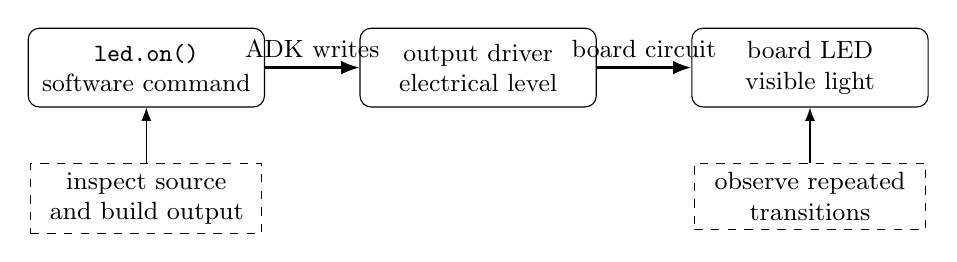
\begin{tikzpicture}[node distance=7mm and 12mm,>=Latex,
 every node/.style={font=\small,align=center}]
    \node[draw,rounded corners,minimum width=3cm,minimum height=1cm] (code)
        {\texttt{led.on()}\\software command};
    \node[draw,rounded corners,minimum width=3cm,minimum height=1cm,
          right=of code] (pin) {output driver\\electrical level};
    \node[draw,rounded corners,minimum width=3cm,minimum height=1cm,
          right=of pin] (light) {board LED\\visible light};
    \draw[->,thick] (code) -- node[above]{ADK writes} (pin);
    \draw[->,thick] (pin) -- node[above]{board circuit} (light);
    \node[draw,dashed,below=of code,text width=2.7cm] (inspect)
        {inspect source and build output};
    \node[draw,dashed,below=of light,text width=2.7cm] (observe)
        {observe repeated transitions};
    \draw[->] (inspect) -- (code);
    \draw[->] (observe) -- (light);
\end{tikzpicture}
\end{center}

\textbf{Important limitation.} Seeing light supports the claim that the visible
indicator changed. It does not independently measure pin voltage, exact
duration, or current. This no-external-wiring lesson intentionally does not
probe those quantities.

\begin{center}
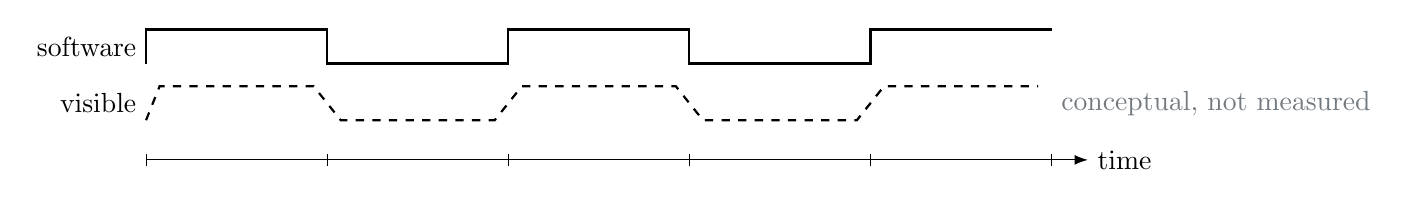
\begin{tikzpicture}[x=1.15cm,y=0.72cm,>=Latex]
    \node[left] at (0,2) {software};
    \node[left] at (0,1) {visible};
    \draw[->] (0,0) -- (10.4,0) node[right]{time};
    \foreach \x in {0,2,...,10}
    {
        \draw (\x,0.1)--(\x,-0.1);
    }
    \draw[thick] (0,1.7)--(0,2.3)--(2,2.3)--(2,1.7)--(4,1.7)
      --(4,2.3)--(6,2.3)--(6,1.7)--(8,1.7)--(8,2.3)--(10,2.3);
    \draw[thick,dashed] (0,0.7)--(0.15,1.3)--(1.85,1.3)--(2.15,0.7)
      --(3.85,0.7)--(4.15,1.3)--(5.85,1.3)--(6.15,0.7)
      --(7.85,0.7)--(8.15,1.3)--(9.85,1.3);
    \node[right,mid] at (10,1) {conceptual, not measured};
\end{tikzpicture}
\end{center}

The dashed visible trace illustrates finite response and perception; it is not
sample data. What observation would weaken the explanation that the program
causes the pattern? For example: the LED continues unchanged after the program
is replaced by a known-dark sketch.

\section*{3. The lifecycle in the supplied program}

\begin{lstlisting}[style=adkcpp]
#include <adk.h>

adk::led::Mono led(LED_BUILTIN);

void setup()
{
    adk::initialize();
}

void loop()
{
    constexpr auto intervalMs = 100;

    led.on  ();
    delay   (intervalMs);

    led.off ();
    delay   (intervalMs);
}
\end{lstlisting}

Opening parentheses are aligned within the logical group. Braces occupy their
own lines, and the ADK component is a \texttt{struct}.

\subsection*{Read the object lifetime, not just the blink}

\begin{center}
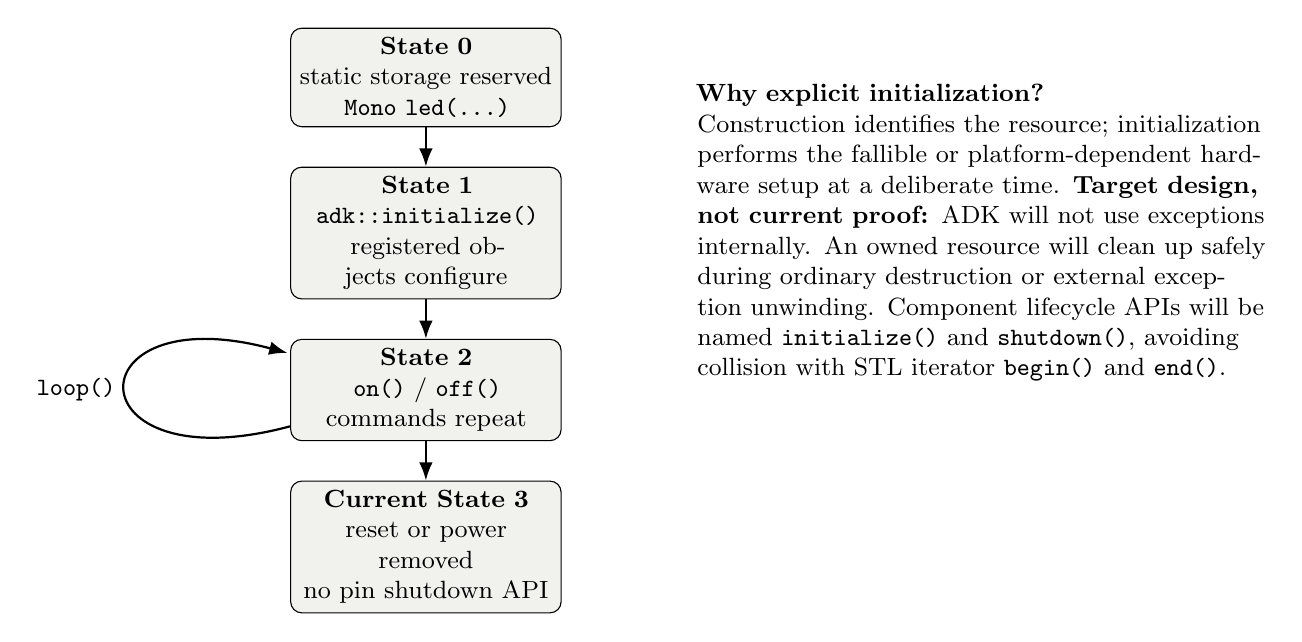
\begin{tikzpicture}[node distance=5mm,>=Latex,every node/.style={font=\small}]
    \node[draw,rounded corners,fill=soft,text width=3.2cm,align=center] (construct)
        {\textbf{State 0}\\static storage reserved\\\texttt{Mono led(...)}};
    \node[draw,rounded corners,fill=soft,text width=3.2cm,align=center,
          below=of construct] (initialize)
        {\textbf{State 1}\\\texttt{adk::initialize()}\\registered objects configure};
    \node[draw,rounded corners,fill=soft,text width=3.2cm,align=center,
          below=of initialize] (command)
        {\textbf{State 2}\\\texttt{on()} / \texttt{off()}\\commands repeat};
    \node[draw,rounded corners,fill=soft,text width=3.2cm,align=center,
          below=of command] (shutdown)
        {\textbf{Current State 3}\\reset or power removed\\no pin shutdown API};
    \draw[->,thick] (construct)--(initialize);
    \draw[->,thick] (initialize)--(command);
    \draw[->,thick] (command) edge[loop left] node[left]{\texttt{loop()}} (command);
    \draw[->,thick] (command)--(shutdown);
    \node[right=16mm of initialize,text width=7.2cm,align=left] {
        \textbf{Why explicit initialization?}\\
        Construction identifies the resource; initialization performs the
        fallible or platform-dependent hardware setup at a deliberate time.
        \textbf{Target design, not current proof:} ADK will not use exceptions
        internally. An owned resource will clean up safely during ordinary
        destruction or external exception unwinding. Component lifecycle APIs
        will be named \texttt{initialize()} and \texttt{shutdown()}, avoiding
        collision with STL iterator \texttt{begin()} and \texttt{end()}.
    };
\end{tikzpicture}
\end{center}

\textbf{Current implementation versus target.} Today, the global
\texttt{adk::initialize()} helper initializes registered objects.
\texttt{Object}'s destructor unregisters an object, but the current pin and LED
types do not yet expose component-level \texttt{shutdown()} or demonstrate
pin-state cleanup. The target RAII design will add idempotent, nonthrowing
cleanup: generic outputs become high-impedance by default and semantic LEDs
become inactive. This lesson demonstrates current initialization and commands;
it does \emph{not} claim that the target cleanup behavior exists yet.

\begin{checkpoint}{explain each line before upload}
\begin{tabularx}{\linewidth}{@{}p{0.28\linewidth}X@{}}
\toprule
Line or construct & Your explanation\\
\midrule
\texttt{LED\_BUILTIN} & \rule{0pt}{0.7cm}\\
\texttt{adk::initialize()} & \rule{0pt}{0.7cm}\\
\texttt{led.on()} & \rule{0pt}{0.7cm}\\
\texttt{delay(intervalMs)} & \rule{0pt}{0.7cm}\\
\bottomrule
\end{tabularx}
\end{checkpoint}

\section*{4. Build without touching the board}

From the repository root, run:
\begin{lstlisting}[style=adkcpp,language=bash]
arduino-cli version
arduino-cli core list
make arduino-001
\end{lstlisting}

The repository defaults \texttt{BOARD\_FQBN} to
\texttt{arduino:avr:mega}. If you override it, record the override. A
successful compile is evidence that the translation and link stages accepted
the program for the selected board; it is not evidence that upload or hardware
behavior succeeded.

\begin{checkpoint}{State 0 --- compile acceptance}
\textbf{Record, do not paraphrase:}\\
\begin{tabularx}{\linewidth}{@{}p{0.31\linewidth}X@{}}
Board/FQBN & \\
Tool version & \\
Final success line & \\
Flash bytes / capacity & \\
RAM bytes / capacity & \\
\end{tabularx}

\textbf{Reject the build} if the board target is not the Mega 2560, compilation
has any error, or size exceeds the reported capacity. Fix that evidence before
uploading.
\end{checkpoint}

\section*{5. Perform and verify: numbered physical states}

\begin{center}
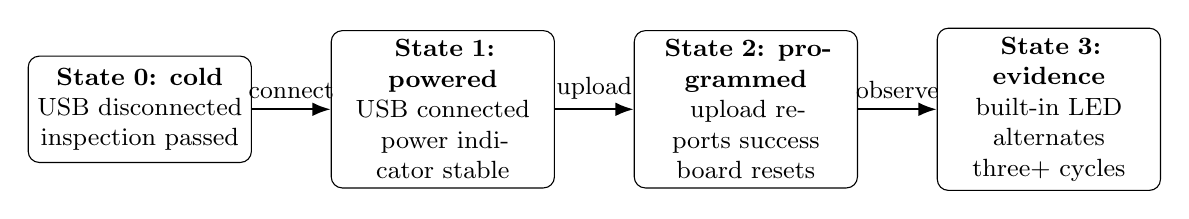
\begin{tikzpicture}[>=Latex,node distance=7mm and 10mm,
 every node/.style={font=\small,align=center}]
    \node[draw,rounded corners,text width=2.6cm,minimum height=1.35cm] (s0)
      {\textbf{State 0: cold}\\USB disconnected\\inspection passed};
    \node[draw,rounded corners,text width=2.6cm,minimum height=1.35cm,
          right=of s0] (s1)
      {\textbf{State 1: powered}\\USB connected\\power indicator stable};
    \node[draw,rounded corners,text width=2.6cm,minimum height=1.35cm,
          right=of s1] (s2)
      {\textbf{State 2: programmed}\\upload reports success\\board resets};
    \node[draw,rounded corners,text width=2.6cm,minimum height=1.35cm,
          right=of s2] (s3)
      {\textbf{State 3: evidence}\\built-in LED alternates\\three+ cycles};
    \draw[->,thick] (s0)--node[above]{connect}(s1);
    \draw[->,thick] (s1)--node[above]{upload}(s2);
    \draw[->,thick] (s2)--node[above]{observe}(s3);
\end{tikzpicture}
\end{center}

\begin{enumerate}
    \item Place the inspected board on a dry, nonconductive surface. Keep all
    headers empty. Verify State 0 against the diagram.
    \item Connect the USB cable. Verify the ordinary power indicator is stable.
    If not, disconnect and stop.
    \item Identify the serial port with the repository's documented listing
    command. Record the exact port: \rule{4cm}{0.35pt}.
    \item Upload with
    \texttt{make upload LESSON=001 PORT=/dev/ttyACM0}, replacing the example
    port with the exact port recorded in step 3. Read the final status; do not
    treat scrolling text as success.
    \item After automatic reset, observe from a comfortable distance. Count
    \emph{complete} bright--dark cycles for 10 s. Repeat three times.
\end{enumerate}

\begin{checkpoint}{intermediate question before interpreting}
Does the LED visibly reach both a brighter and a darker state? \(\square\) yes
\(\square\) no. Does the upload tool explicitly report success?
\(\square\) yes \(\square\) no.

If either answer is no, do not fill the acceptance claim yet; use the
troubleshooting table.
\end{checkpoint}

\begin{table}[h]
\centering
\caption{Direct observations. Enter your data; the expected pattern is not sample data.}
\begin{tabularx}{\linewidth}{@{}c>{\centering\arraybackslash}p{0.16\linewidth}
>{\centering\arraybackslash}p{0.17\linewidth}X@{}}
\toprule
Trial & Observation time (s) & Complete cycles & Notes: brightness, irregularity, reset\\
\midrule
1 & 10 & & \rule{0pt}{0.85cm}\\
2 & 10 & & \rule{0pt}{0.85cm}\\
3 & 10 & & \rule{0pt}{0.85cm}\\
\bottomrule
\end{tabularx}
\end{table}

Mean observed count:
\[
\bar n=\frac{n_1+n_2+n_3}{3}
=\frac{\rule{0.8cm}{0.35pt}+\rule{0.8cm}{0.35pt}+\rule{0.8cm}{0.35pt}}{3}
=\rule{1.5cm}{0.35pt}\ {\rm cycles\ per\ 10\,s}.
\]
Range \(=\max(n)-\min(n)=\rule{1.2cm}{0.35pt}\) cycles.

\section*{6. Diagnose by symptom, with a safe next check}

\begin{tabularx}{\linewidth}{@{}p{0.20\linewidth}p{0.28\linewidth}X@{}}
\toprule
Symptom & Plausible cause & Safe next check\\
\midrule
No power indicator & Charge-only/damaged cable, bad USB port, damaged board &
Disconnect. Inspect and try one known-good data cable and host port. Stop if
heat, odor, or repeated disconnect occurs.\\
Port absent & Permissions, cable, or device enumeration & Keep headers empty.
Run the port-listing command before and after connection; compare the lists.
Do not guess a device path.\\
Compile fails & Wrong target, missing core, source/API mismatch & Stay
disconnected. Record the first error, selected FQBN, and tool versions. Fix the
first error before upload.\\
Upload fails & Wrong port/FQBN, port in use, cable problem & Do not repeatedly
reset. Confirm Mega 2560 target, close serial monitors, re-list ports, retry
once with recorded settings.\\
Upload succeeds; LED dark & Wrong observable LED, command not reached, board
variant, hardware fault & Press reset once and watch from reset onward.
Re-read \texttt{LED\_BUILTIN}; upload a known-good built-in-LED example only as
a controlled comparison.\\
LED steady & Blink too fast to resolve, stale program, reset loop & Confirm the
reported upload artifact and port. Change only the interval to 1000 ms for the
extension; observe whether clear transitions appear.\\
Irregular pattern & Reset, unstable USB, host connection, observation error &
Check whether power indicator or serial connection also resets. Repeat a
timed trial without touching cable or board.\\
\bottomrule
\end{tabularx}

\textbf{Escalate rather than improvise} when two known-good cables/ports still
cannot enumerate the board, a known-good example cannot control the built-in
LED, physical damage is visible, or any electrical stop condition occurs.

\section*{7. Controlled extension: change one variable}

Change only the interval from 100 ms to 1000 ms. Keep the same board, port,
cable, component, sequence, observer, and 10 s observation window.

\begin{lstlisting}[style=adkcpp]
constexpr auto intervalMs = 1000;
\end{lstlisting}

\begin{center}
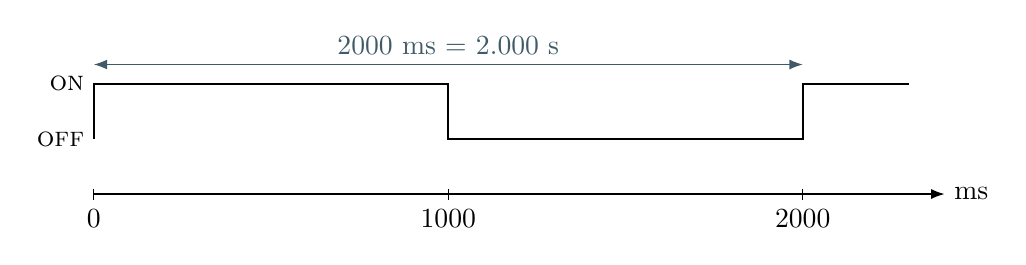
\begin{tikzpicture}[x=0.0045cm,y=0.7cm,>=Latex]
    \draw[->] (0,0)--(2400,0) node[right]{ms};
    \draw[thick] (0,1)--(0,2)--(1000,2)--(1000,1)--(2000,1)--(2000,2)--(2300,2);
    \node[left] at (0,2) {\textsc{on}};
    \node[left] at (0,1) {\textsc{off}};
    \draw[<->,accent] (0,2.35)--node[above]{2000 ms = 2.000 s}(2000,2.35);
    \foreach \x/\lab in {0/0,1000/1000,2000/2000}
    {
        \draw (\x,0.1)--(\x,-0.1) node[below]{\lab};
    }
\end{tikzpicture}
\end{center}

Before uploading, predict the new frequency:
\[
f=\frac{1}{(1000+1000)\ {\rm ms}}
=\rule{1.5cm}{0.35pt}\ {\rm Hz}.
\]

\begin{tabularx}{\linewidth}{@{}p{0.22\linewidth}p{0.22\linewidth}
p{0.22\linewidth}X@{}}
\toprule
Condition & Predicted cycles / 10 s & Observed cycles / 10 s & What changed perceptually?\\
\midrule
100 ms interval & & & \rule{0pt}{0.75cm}\\
1000 ms interval & & & \rule{0pt}{0.75cm}\\
\bottomrule
\end{tabularx}

\textbf{Controlled-comparison inference:} If the longer interval creates fewer,
more easily distinguished transitions, the changed interval is the leading
explanation because the other named variables were held constant. It is not
proof that every timing source is exact.

\section*{8. Assessment: can you transfer the method?}

\textbf{A. Label the states.} Write \textsc{commanded on},
\textsc{commanded off}, or \textsc{transition} beneath each marked point.

\begin{center}
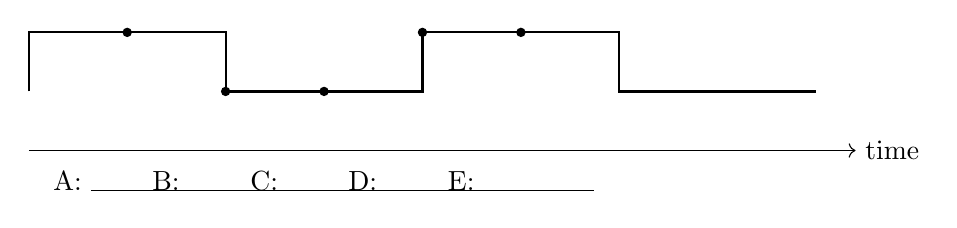
\begin{tikzpicture}[x=1.25cm,y=0.75cm]
    \draw[->] (0,0)--(8.4,0) node[right]{time};
    \draw[thick] (0,1)--(0,2)--(2,2)--(2,1)--(4,1)--(4,2)--(6,2)--(6,1)--(8,1);
    \foreach \x/\lab in {1/A,2/B,3/C,4/D,5/E}
    {
        \fill (\x,{ifthenelse(mod(\x,4)==1 || mod(\x,4)==0,2,1)}) circle (1.7pt);
        \node[below] at (\x,-0.2) {\lab: \rule{1.4cm}{0.3pt}};
    }
\end{tikzpicture}
\end{center}

\textbf{B. Calculate.} For 250 ms on and 750 ms off, calculate period,
frequency, and duty fraction. Keep units visible.

\vspace{1mm}
\blankline\\[9pt]\blankline\\[9pt]\blankline

\textbf{C. Separate evidence from inference.} Mark each statement O
(observation), I (inference), or U (unsupported by this lesson).

\begin{tabularx}{\linewidth}{@{}p{0.06\linewidth}X@{}}
\rule{0.6cm}{0.35pt} & The visible LED alternated between brighter and darker states.\\
\rule{0.6cm}{0.35pt} & Exactly 5.000000 cycles occurred every second.\\
\rule{0.6cm}{0.35pt} & The uploaded program is a plausible cause of the repeated pattern.\\
\rule{0.6cm}{0.35pt} & The output pin delivered a measured 5.00 V.\\
\end{tabularx}

\textbf{D. Lifecycle.} Why is \texttt{initialize()}/\texttt{shutdown()} clearer
for hardware ownership than \texttt{begin()}/\texttt{end()} in a C++ library?

\blankline\\[9pt]\blankline

\textbf{E. Falsification.} Name one result that would weaken your explanation
that the ADK commands caused the visible pattern.

\blankline\\[9pt]\blankline

\section*{9. Final acceptance proof: Claim--Evidence--Reasoning}

\textbf{Acceptance criteria}

\checkbox\ cold inspection passed \quad
\checkbox\ Mega 2560 target recorded \quad
\checkbox\ compile and upload explicitly succeeded

\checkbox\ both visible states observed \quad
\checkbox\ three timed trials recorded \quad
\checkbox\ controlled extension changed only the interval

\textbf{Claim.} State narrowly what this build demonstrated. Do not claim
voltage or exact timing unless independently measured.

\vspace{1mm}\blankline\\[9pt]\blankline\\[9pt]\blankline

\textbf{Evidence.} Cite your upload result, repeated counts (with units), and
controlled comparison.

\vspace{1mm}\blankline\\[9pt]\blankline\\[9pt]\blankline\\[9pt]\blankline

\textbf{Reasoning.} Explain why those observations support the claim and why
the one-variable comparison matters.

\vspace{1mm}\blankline\\[9pt]\blankline\\[9pt]\blankline\\[9pt]\blankline

\textbf{Uncertainty and alternatives.} State at least one limitation (human
counting, oscillator tolerance, hidden board circuitry, reset behavior) and
one plausible competing explanation.

\vspace{1mm}\blankline\\[9pt]\blankline\\[9pt]\blankline

\begin{center}
\fbox{\begin{minipage}{0.92\linewidth}
\textbf{Lesson complete only when the evidence survives review.}
A reviewer should be able to reconstruct what target was built, what was
observed, how often it was repeated, what variable changed, and what would
cause rejection. A bright LED by itself is an event; a documented,
repeatable comparison is evidence.
\end{minipage}}
\end{center}

\section*{Instructor / reviewer key}

\small
Expected values: 100 ms case \(T=200\ {\rm ms}=0.200\ {\rm s}\),
\(f=5.00\ {\rm Hz}\), approximately 50 cycles in 10 s; 1000 ms case
\(T=2.000\ {\rm s}\), \(f=0.500\ {\rm Hz}\), approximately 5 cycles in 10 s.
Assessment B: \(T=1.000\ {\rm s}\), \(f=1.00\ {\rm Hz}\), duty fraction
\(250/1000=0.250=25.0\%\). Assessment C: O, U, I, U.
Accept reasonable variation in hand counts only when the learner names the
uncertainty. Reject a CER that substitutes expected values for recorded
observations, claims a measured voltage, or omits the controlled comparison.

\textbf{Asset provenance note.} The graphite orientation plate is the
project-provided asset
\texttt{001-built-in-led-pencil.png}, reviewed here only
for board/cable/light orientation. It is not authoritative for component
placement, pin identity, dimensions, or electrical topology. All timing,
state, lifecycle, and acceptance logic in this publication is rendered as
deterministic TeX/TikZ.

\end{document}
